\chapter{Information and Communication Technologies for Developing Countries}
\section{In General}
No correlation with productivity \cite{rh:isdc}
\subsection{Objective}
\subsubsection{Productivity}
\subsubsection{Allocation of resources}
\subsubsection{Decision making}

\begin{quotation}
Lack of literature in general: Until very recently,
the entire literature on IS and developing countries
would struggle to ll a single bookshelf. The
attention of writers—from researchers to consultants
to journalists—has been focused elsewhere.\cite{rh:isdc}
\end{quotation}
\begin{quotation}
Lack of evaluation: Those who have the will to
evaluate—such as academics—often lack the
resources and capacity. Those who have the
resources—such as aid donor agencies—often
lack the will to evaluate.\cite{rh:isdc}
\end{quotation}
\begin{quotation}
Focus on case studies: The literature on IS in
DCs has grown, but it is a literature dominated by
case studies of individual IS projects. Taken alone,
these provide no basis for estimation of overall
failure/success rates.\cite{rh:isdc}
\end{quotation}

\section{Discourses}
Chrisanthi \cite{ca:isdc} points out three main branches that characterizes implementation of information systems in developing countries.
\subsection{Diffusion}
Just move the technology and understanding to a new place. Usually from I-countries to D-countries.Usually a mismatch between actuality and design.
\subsection{Transformative}
Transforming the organization to operate in a new way with the technology. (My understanding should be confirmed.)
Working towards a design while facilitating the design-actuality gap. The whole is seen as a process with a starting point and an end point.
\subsection{Socially Embedded}
Building the competence and technology from the ground up by including locals. User participation. Making the design and actuality gap smaller. 

Diffusion and transformative development does not facilitate the already existing structures of the context the technology will be placed within.
The implementation of information systems from this perspective requires the environment and the people in it to adapt to the new technology.
This will in turn increase the risk of the information system being rejected by the users. On the other hand, the socially embedded path
will to some extent safeguard the underlying social structures by building upon what is already there. 
This might lead to unexpected results and be time consuming. Although, probably avoiding the sustainability pitfall.

\section{Pitfalls in introducing IS in Developing Countries}
\subsection{Scalability}
The problem of moving expertise and system to new locations with the lessons learned.
By conceptualize the use of ICT's one can make it easier to transfer ICT's to other locations, making it scalable.\cite{jbemss:noa}.
\subsection{Sustainability}
What happens when the AID funded projects stops being funded? The donors are interested in sustainable solutions that keep existing after the investment.
How does one maintain a project that is built on temporary donors. Unfortunately many IS projects are drained from resources \cite{ca:isdc}.
Here should it be mentioned something about political commitment \cite{jbemss:noa}.  

\subsection{Assimilation In Dysfunctional Organizational Processes}
One has to take into account that an already broken system can't be fixed by speeding it up.
Automating a process that already does not produce the right result would only give us more of the result we are trying to change \cite{mh:rw}.

\subsection{Lack of persistence on key areas}

\section{Updated Information}

\section{The design and actuality gap}


\section{Success or Failure}

\begin{figure}
\centering
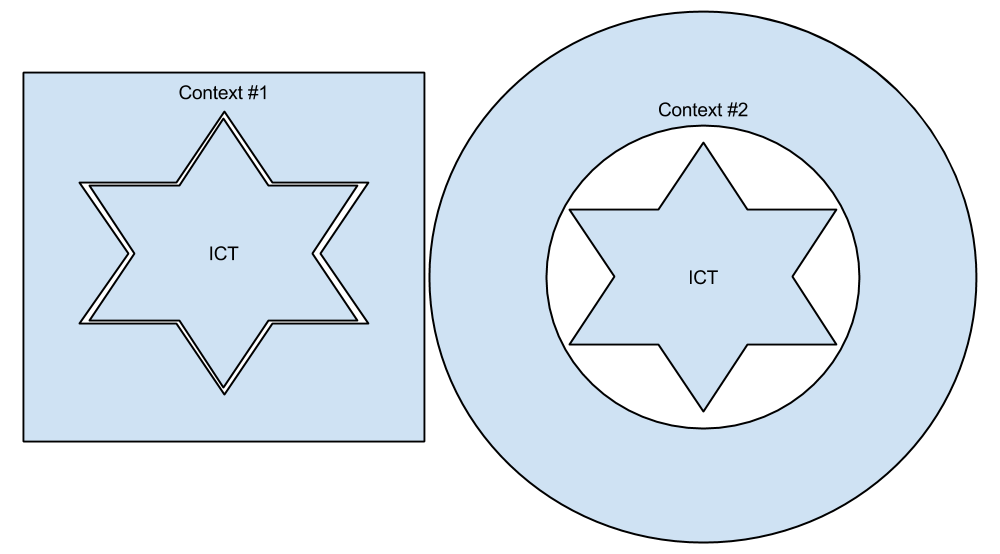
\includegraphics[width=\columnwidth]{literature/ict_in_dev/images/contextIctProblem.png}
\label{cip}
\caption{If it works for us it will work for you!}
\end{figure}


\begin{figure}
\centering
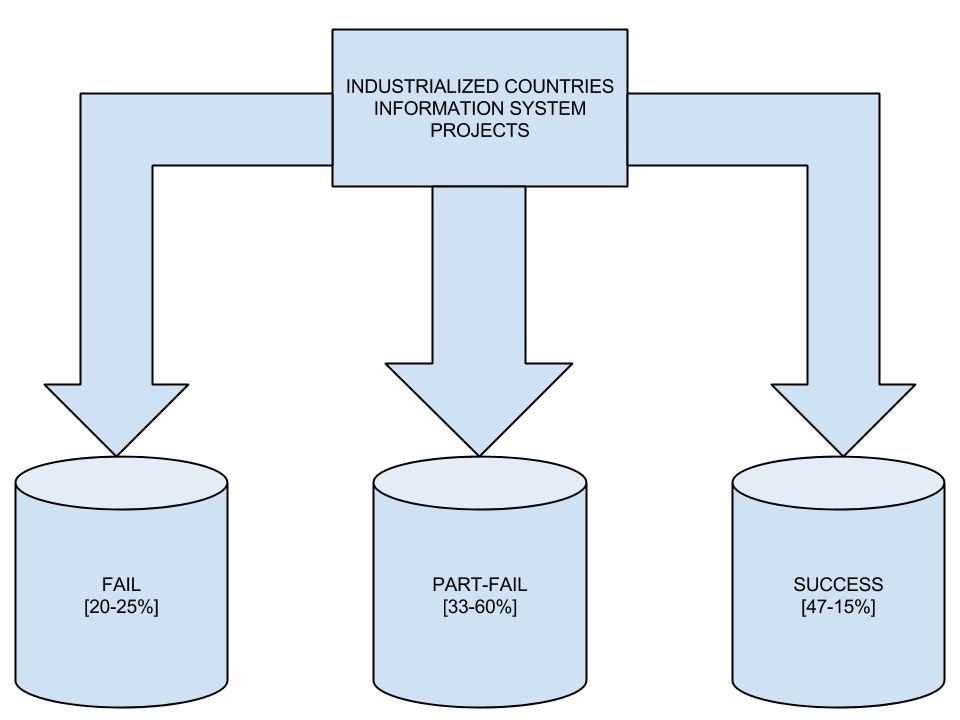
\includegraphics[width=\columnwidth]{literature/ict_in_dev/images/iCountryISProjects(1995-2000).png}
\label{icisp}
\caption{IS projects in Industrialized Countries. Year: 1995-2000 \cite{rh:isdc}}
\end{figure}


\section{Success stories}
\subsection{short examples}
\section{Failure stories}
\subsection{short examples}

\section{Evidence base}

\begin{quotation}
Health information systems in South Africa: Braa
and Hedberg (2002) reported widespread partial
failure of high cost systems with little use of data.\cite{rh:isdc}
\end{quotation}

\begin{quotation}
IS in the Thai public sector: Kitiyadisai (2000)
reported “failure cases seem to be the norm in
Thailand at all governmental levels.”\cite{rh:isdc}
\end{quotation}

\begin{quotation}
Donor-funded IT projects in China: Baark and
Heeks (1999) reported that all were found to be
partial failures.\cite{rh:isdc}
\end{quotation}

\begin{quotation}
World Bank-funded IT projects in Africa: Moussa
and Schware (1992) reported almost all as partial—
often sustainability—failures.\cite{rh:isdc}
\end{quotation}


\section{Digital Divide}

\section{Implicit and explicit components of Design}
The explicit components of a computer application is the physical components the user would need in order to use the application.
Examples include cost, computer hardware, operating system, monitor and such.
The implicit ones are a little harder to quantify. These include knowledge, expectations and skill.
When addressing the implicit, how would one go about evaluating if the user is qualified to use the application as intended and ensure that it is used for the proper intentions?  

\section{Outsourcing}
IS has the potential of being more than just a tool for making processes better, more efficient etc.
With enough knowledge a country may provide a service in the form of providing ICT solutions and support. Rwanda being a good example.
Knowledge is key, it requires little more than effort and some hardware, making it possible for 
countries with little natural resources to have the opportunity to contribute to the global market.
India is currently being a great example of this. 

\section{Education and IS development}

\section{Untapped Marked}
From a certain perspective one can see the developing countries as an untapped marked.
By building up the countries infrastructure one has the opportunity to offer services that previously was not possible.
Take Telenor and their agenda to offer insurance and banking services in the east.
By building up the infrastructure they can now offer their services as "mobile providers" and even expand their services to banking with a fresh market and less competition.

\section{IT and Economic Growth}
With IT comes the assumption that it will in some way enable economic growth \cite{ca:ieeg}.
Although it can be said that highly successful businesses is using IT it would be wrong to say that more IT equals more money.
For an example.
The simple view of IT being able to enable economic growth is not enough.
It can however increase productivity in several ways by automating existing processes, but the potential of IT lies in new ways of structuring organizations.
Time and space can be compromised significantly.

In the 1980's there was invested 750 billion \$ in IT \cite{ca:ieeg}, but this only lead to \(0.7\%\) increase in productivity. This was a decrease from the previous decade.
There is findings that suggests that ICT has a positive correlation with productivity. Data from 1983 to 1990 shows this for eleven Asia pacific countries \cite{ca:ieeg}. May be a necessity in order to take part in the global economy and making it possible to trade. IT can also directly affect how organizations structure themselves by introducing new ways of working and increasing productivity.
ICT should be used is withing the organization to enable better work processes, not automatize existing processes \cite{mh:rw}. 

\section{Sustainability\cite{jbemss:noa}}

Building networks running on the same concept will make the ICT initiative more sustainable. 

User participation is another tool one can use in order to make ICT initiative more sustainable.
When the concept is accepted and made by the users they understand how and why it works and are more likely to accept it.
